%!TEX root = ../greb.tex
% Тип документа
\documentclass[a4paper,12pt]{extarticle}

% Шрифты, кодировки, символьные таблицы, переносы
% \usepackage{cmap}
% \usepackage[T2A]{fontenc}
\usepackage[utf8]{inputenc}
\usepackage[russian]{babel}
% Это пакет -- хитрый пакет, он нужен но не нужен
\usepackage[mode=buildnew]{standalone}

\usepackage
	{
		% Дополнения Американского математического общества (AMS)
		amssymb,
		amsfonts,
		amsmath,
		amsthm,
		% Пакет для физических текстов
		physics,
		% misccorr,
		% 
		% Графики и рисунки
		wrapfig,
		graphicx,
		subcaption,
		float,
		tikz,
		tikz-3dplot,
		caption,
		csvsimple,
		color,
		booktabs,
		geometry,
		% 
		% Таблицы, списки
		makecell,
		multirow,
		indentfirst,
		%
		% Интегралы и прочие обозначения
		ulem,
		esint,
		esdiff,
		% 
		% Колонтитулы
		fancyhdr,
	} 
    
\usepackage{mathtools}
\mathtoolsset{showonlyrefs=true} 
\usepackage{pgfplots,pgfplotstable,booktabs,colortbl}
\usepackage{xcolor}
\usepackage{hyperref}
\usepackage{pythontex}
 % Цвета для гиперссылок
\definecolor{linkcolor}{HTML}{000000} % цвет ссылок
\definecolor{urlcolor}{HTML}{799B03} % цвет гиперссылок
 
\hypersetup{pdfstartview=FitH,linkcolor=linkcolor,urlcolor=urlcolor, colorlinks=true}
\hypersetup{pageanchor=false}
% Увеличенный межстрочный интервал, французские пробелы
\linespread{1.3} 
\frenchspacing 

\newcommand{\mean}[1]{\langle#1\rangle}

\begin{pycode}
##
def frexp10(decimal):
	parts = ('%e' % decimal).split('e')
	return float(parts[0]), int(parts[1])
##
\end{pycode}



% Функция для тех, кто использует pythontex. Представляет любое вещественное число в стандартном виде.
\newcommand{\frexp}[1]{
		\pyc{#10=frexp10(#1)} 
			\py{ round(#10[0],2)} 
				\cdot 10^{\py{#10[1]}} }

% const прямым шрифтом
\newcommand\ct[1]{\text{\rmfamily\upshape #1}}
\newcommand*{\const}{\ct{const}}
\usepackage{array}
\usepackage{pstool}

\geometry		
	{
		left			=	2cm,
		right 			=	2cm,
		top 			=	2.5cm,
		bottom 			=	2.5cm,
		bindingoffset	=	0cm
	}

%%%%%%%%%%%%%%%%%%%%%%%%%%%%%%%%%%%%%%%%%%%%%%%%%%%%%%%%%%%%%%%%%%%%%%%%%%%%%%%
	%применим колонтитул к стилю страницы
\pagestyle{fancy} 
	%очистим "шапку" страницы
% \fancyhead{} 
	%слева сверху на четных и справа на нечетных
\fancyhead[R]{}%\labauthors 
	%справа сверху на четных и слева на нечетных
% \fancyhead[L]{Отчёт по лабораторной работе №\labnumber}
\fancyhead[L]{\labtheme} 
	%очистим "подвал" страницы
% \fancyfoot{} 
	% номер страницы в нижнем колинтуле в центре
\fancyfoot[C]{\thepage} 

%%%%%%%%%%%%%%%%%%%%%%%%%%%%%%%%%%%%%%%%%%%%%%%%%%%%%%%%%%%%%%%%%%%%%%%%%%%%%%%

\renewcommand{\contentsname}{Оглавление}
\usepackage{tocloft}
\usepackage{secdot}
\sectiondot{subsection}


\begin{document}
\def\labauthors{Виноградов И.Д., Понур К.А., Шиков А.П.}
\def\labgroup{440}
\def\labnumber{1}
\def\labtheme{Исследование твердотельных структур методом ЭПР-спектроскопии}
\def\department{Кафедра квантовой радиофизики и электроники}
\begin{titlepage}

\begin{center}

{\small\textsc{Нижегородский государственный университет имени Н.\,И. Лобачевского}}
\vskip 1pt \hrule \vskip 3pt
{\small\textsc{Радиофизический факультет}}



\vfill
{\Large {\department}}

{\Large Отчет по лабораторной работе №\labnumber\vskip 12pt\bfseries \labtheme}
	
\end{center}

\vfill
	
\begin{flushright}
	{Выполнили студенты \labgroup\ группы\\ \labauthors}%\vskip 12pt Принял:\\ Менсов С.\,Н.}
\end{flushright}
	
\vfill
	
\begin{center}
	Нижний Новгород, \the\year
\end{center}

\end{titlepage}


\newpage
\section{Теоретическая часть}%
В данной работе проводится исследование спектров поглощения ЭПР двух твердотельных структур: свободного радикала \textbf{дифенила} и парамагнитного кристаллического вещества --
\textbf{рубина}. Рассмотрим качественную картину спектров данных образцов.
\paragraph{Дифенил} представляет собой сложную по своей структуре молекулу с молярным весом в 518, имеющую один неспаренный электрон. Его парамагнетизм обусловлен спиновым моментом неспаренного электрона. У дифенила будет наблюдаться только один резонансный переход, и сигнал ЭПР будет представлять собой одиночную резонансную линию.
\paragraph{Рубин}%
представляет собой кристалл корунда $Al_2 O_3,$ в котором часть ионов  $Al^{3+}$ замещена парамагнитными ионами  $Cr^{3+}$ с суммарным спином  $S = \frac{3}{2}$. 
Результирующий ЭПР-спектр рубина определяется числом разрешенных резонансных переходов, для которых выполняется соотношение $E_m-E_{m'} = \hbar \omega$. 
Разрешенными переходами будут такие, для которых матричный элемент  дипольного момента $\mu_{mm'}$ не равен 0.
В конечном счете, вычисление матричного элемента $\mu_{mm'}$ сводится к следующему:
\begin{equation}
    \label{eq:51}
    \mu_{mm'} = \frac{g \beta_B}{\hbar} \mel{m}{\hat S_x}{m'} 
\end{equation}

Для его вычисления используют операторы повышения и понижения
\begin{gather}
    \hat S_+ = \hat S_x + i \hat S_y; \\
    \hat S_- = \hat S_x -  i \hat S_y
\end{gather}

Заменяя в \eqref{eq:51} оператор $\hat S_x$ на  $\frac{\hat S_+ + \hat S_-}{2} $ можно убедиться в том, что отличными от нуля будут только матричные элементы вида
$\mel{m}{\hat S_x}{m \pm 1}$. Следовательно, резонансные переходы разрешены только между теми уровнями, квантовые числа  $m$ которых различаются на  $\pm 1$. Всего таких переходов в 
кристалле рубина -- три.


\subsection{Условия выделения кривых и дисперсии на детекторе}%


Волноводный отражательный резонатор с отверстием связи можно представить в виде эквивалентного колебательного контура, импеданс которого определяется выражением
\begin{equation}
    \label{eq:1}
    Z = R + i [ \omega L_{0} - \frac{1}{\omega C}],
\end{equation}
где $R$, $L_{0}$ и $С$ -- эквивалентные сопротивление, индуктивность и ёмкость соответственно. При наличии парамагнетика с магнитной проницаемостью  $\mu$ индуктивность резонатора будет записывать как $L = \mu L_{0}$. При частичном заполнении резонатора образцом магнитная проницаемость выражается через восприимчивость $\chi$ следующим образом
\begin{equation}
    \label{eq:2}
    \mu = 1 + 4 \pi \eta \chi,
\end{equation}
где $\chi$ -- коэффициент заполнения резонатора парамагнетиком. В результате получаем
\begin{equation}
    \label{eq:3}
    Z = R + i \frac{L_{0}}{\omega} \qty( \omega^{2} - \frac{1}{L_{0}C}) + i \omega L_{0} \cdot 4 \pi \eta \chi.
\end{equation} 

Величина $\frac{1}{\sqrt{L_{0} C}}$ дает собственную частоту резонатора. При резонансе $\omega^2 = \frac{1}{L_{0}C} = \omega^2_0$ и выражение для $Z$ принимает вид
\begin{equation}
    \label{eq:4}
    Z = R + i \omega L_{0} \cdot 4 \pi \eta \chi = R \qty( 1 + i 4 \pi \eta \chi' Q + 4 \pi \eta'' Q),
\end{equation}
где $Q = \frac{\omega L_0}{R}$ - добротность резонатора. Если обозначить характеристическое сопротивление волновода через $Z_0$, то комплексный коэффициент отражения от резонатора  $\Gamma$, определяемый как отношение амплитуды падающего на резонатор поля  $E_n$ к амплитуде отраженного поля, будет равен
 \begin{equation}
    \label{eq:5}
    \Gamma = \frac{Z-Z_{0}}{Z+Z_{0}}
\end{equation}

С учётом этого отраженную от резонатора сигнальную волну в точке детектирования можно записать в виде 
\begin{equation}
    \label{eq:6}
    E_{1} = \abs{E_n} \cdot \Gamma \cdot e^{- i 4\pi \frac{L_{1}}{\lambda}},
\end{equation}
где $L_{1}$ -- длина волноводного плеча от детектора до резонатора. Кроме этой волны на детектор поступает сигнал, отраженный ль балансного плеча
\begin{equation}
    \label{eq:7}
    E_{2} = \alpha^2 \abs{E_n} e^{-i 4 \pi \frac{L_{2}}{\lambda}},
\end{equation}
где $\alpha$ - коэффициент ослабления аттенюатора, а  $L_{2}$ -- соответствующая длина балансного плеча. Суммарное поле на детекторе получим в следующем виде:
\begin{equation}
    \label{eq:8}
    E = \abs{E_n} \cdot e^{-i4\pi \frac{L_{1}}{\lambda}} \cdot \qty{\Gamma + \alpha^2 e^{ - i 4 \pi \frac{L_{2} - L_{1}}{\lambda} } }.
\end{equation}

При малых уровнях СВЧ-мощности ток детектора пропорционален квадрату напряженности поля $E$ в этом случае имеем
\begin{equation}
    \label{eq:9}
    i_{\text{дет}} = S \abs{E}^2 = SP_n \cdot \abs{\Gamma + \alpha^2 e^{- i 4 \pi \frac{L_{2}- L_{1}}{\lambda}}   }^2,
\end{equation}
где $S$ -- коэффициент преобразования детектора, а $P_n$ -- мощность, падающая на резонатор. 
Используя неравенства $\chi' \ll 1$,  $\chi'' \ll 1$ и условие хорошей согласованности волновода с резонатором, получаем вид сигнала ЭПР:
\begin{equation}
    \label{eq:14}
    i_{\text{дет}}  = S P_n \cdot 4 \pi Q \eta \qty[ \chi'' \cos(\frac{4 \pi}{\lambda} \Delta L) - \chi' \sin(\frac{4 \pi}{\lambda} \Delta L)]
\end{equation}

Отсюда следует, что в зависимости от положения замыкающего поршня  балансного плеча сигнал на выходе детектора может быть пропорционален либо $\chi'$, либо  $\chi''$. При 
разности $\Delta L = L_{2} - L_{1}$, кратной $\frac{\lambda}{4}$, ток детектора будет пропорционален $\chi''$, а при дополнительном сдвиге на  $\frac{\lambda}{8}$ -- пропорционален кривой $\chi'$.

\subsection{Определение числа парамагнитных частиц в образце}%
\label{sub:2}

Чтобы получить соотношение, позволяющее определить число  парамагнитных частиц исходя из характеристики наблюдаемого сигнала ЭПР, воспользуемся выражением \eqref{eq:14}. При $\Delta L \simeq \frac{\lambda}{4}$ имеем
\begin{equation}
    \label{eq:15}
    i_{\text{дет}} \simeq S P_n \cdot 4 \pi Q \eta \chi''.
\end{equation}

Введем технический коэффициент $A$, характеризующий коэффициент усиления тракта <<детектор-усилитель-осциллограф>>. Его величину можно измерить, подавая известный по величине модулированный СВЧ-сигнал на детекторную головку и измеряя при этом амплитуду видеосигнала на экране осциллографа. Если обозначить через  $L_M$ высоту видеосигнала модуляции 
на экране, а $P_M$ -- величину модулированной компоненты СВЧ-мощности, то коэффициент усиления $A$ будет равен  $\frac{L_M}{P_M}$. Если учесть такого рода амплитудную калибровку, высота сигнала ЭПР на экране осциллографа может быть записана как
\begin{equation}
    \label{eq:16}
    L_{C} = A P_n \cdot 4 \pi Q \eta \chi''(\omega_{0})
\end{equation}

Коэффициент заполнения $\eta$ определяется как отношение  двух интегралов вида  $\int H_{1}^2 \dd{\nu}$ по объему образца и резонатора соответственно. В условиях данной ЭПР-установки
с достаточной степенью точности можно считать 
\begin{equation}
    \label{eq:17}
    \eta \simeq \frac{2 V_{\text{обр}}}{V_{\text{рез}}}.
\end{equation}

Значение $\chi''$ для малых полей  $H_{1}$ при $\omega = \omega_{0}$ можно записать в виде
\begin{equation}
    \label{eq:18}
    \chi '' (\omega_{0}) = \frac{N_{0} \mu^2}{3KT} \omega_{0} T_2^*
\end{equation}
Отсюда количество парамагнитных частиц можно оценить как
\begin{equation}
    \label{eq:20}
    N_0 = 3KT \frac{\chi''(\omega_{0})}{\mu^2 \omega_0 T_2^*}.
\end{equation}
Сопоставляя \eqref{eq:16} и \eqref{eq:20} получаем окончательно
\begin{equation}
    \label{eq:21}
    N_0 = \frac{3KT}{8\pi Q \mu^2 \omega_{0} T_2^*} \cdot \frac{L_C}{L_M}  \cdot \frac{P_M}{P_n} \cdot \frac{V_{\text{рез}}}{V_{\text{обр}}}
\end{equation}
\section{Экспериментальная часть}%


\subsection{Исследование ЭПР в молекулах дифенила}%
\begin{figure}[h!]
    \centering
    \includegraphics[scale=0.8]{example-image-a}
    \caption{Принципиальная схема установки}
    \label{fig:1}
\end{figure}
\paragraph{Получение на экране осциллографа кривых поглощения и дисперсии сигнала ЭПР.}%
\label{par:1}
Для исследования ЭПР в молекулах дифенила, образец был помещен в резонатор, и произведена первоначальная настройка
установки. Клистронный генератор был настроен на центр одной из зон по максимуму мощности ($\nu = 8.96$ ГГц при $\alpha = 0$), а
резонаторная камера была настроена в резонанс (соотв. минимуму сигнала при $\alpha = 1$).

При подключенном к выходе детектора был включен источник постоянного тока для магнитных катушек. Поле $H_0$ было выведено на
резонансное значение $H_0 = 3547$ Гс (при значении тока $I_0 = 160$ мА). Момент резонанса был определен по характерной
наблюдаемой осциллограмме (см. рис. \ref{fig:2}(а)).
\begin{figure}[h!]
    \centering
    \includegraphics[scale=0.33]{example-image-a}
    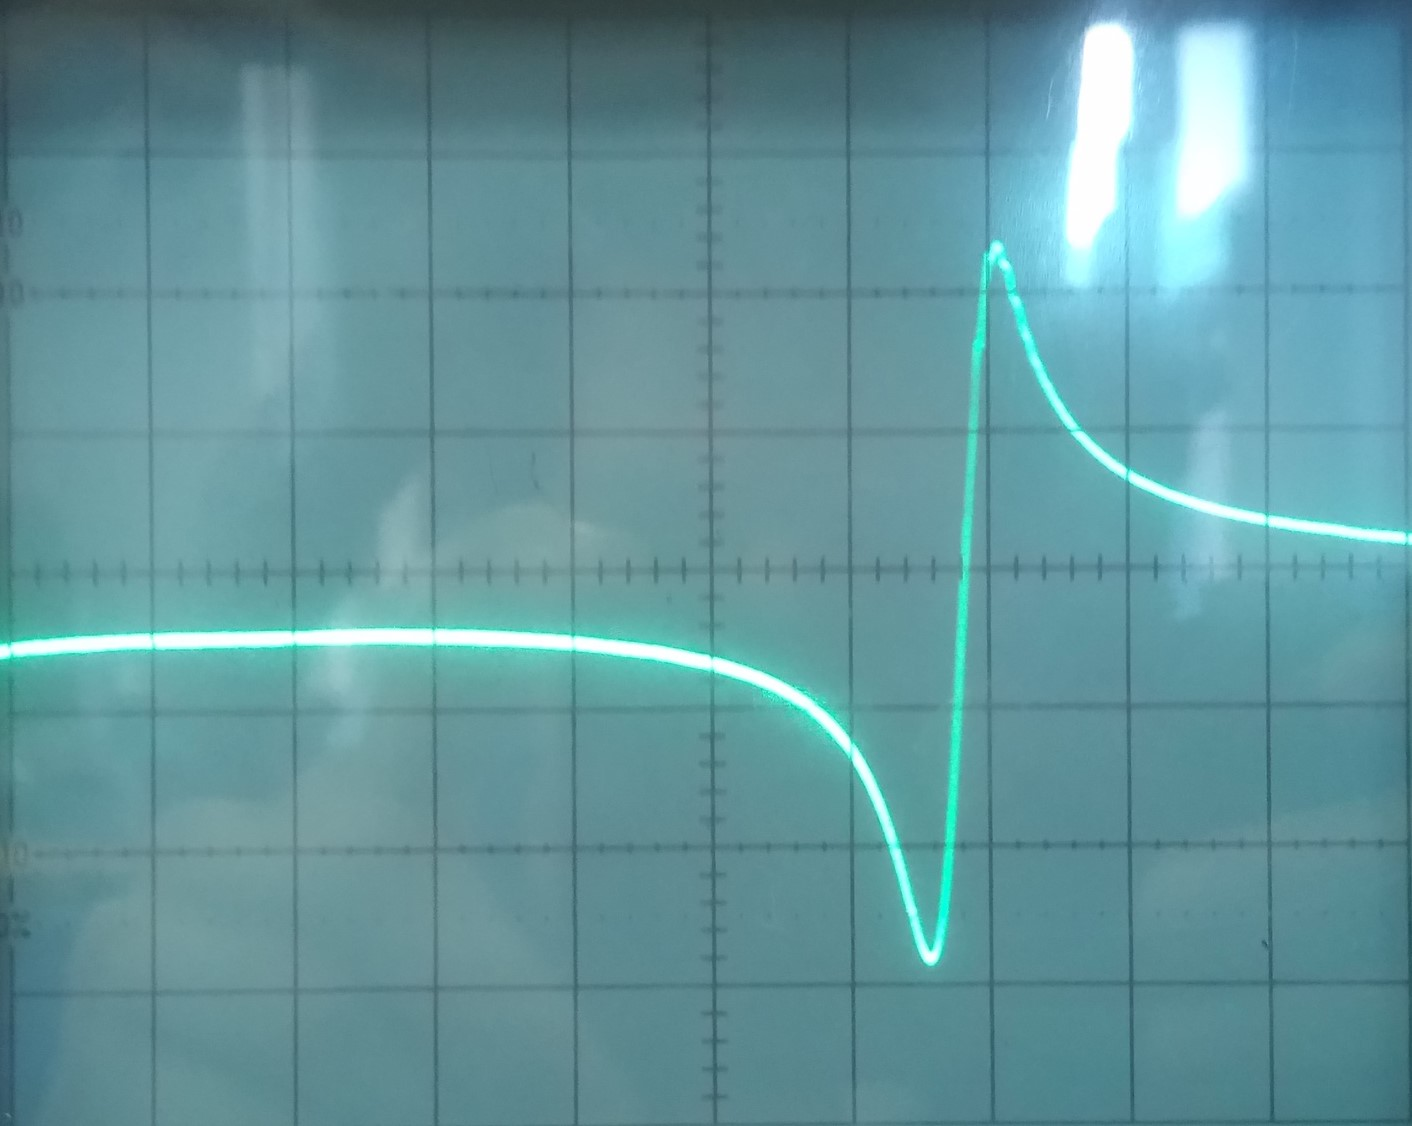
\includegraphics[width=0.3\linewidth]{fig/fig2}
    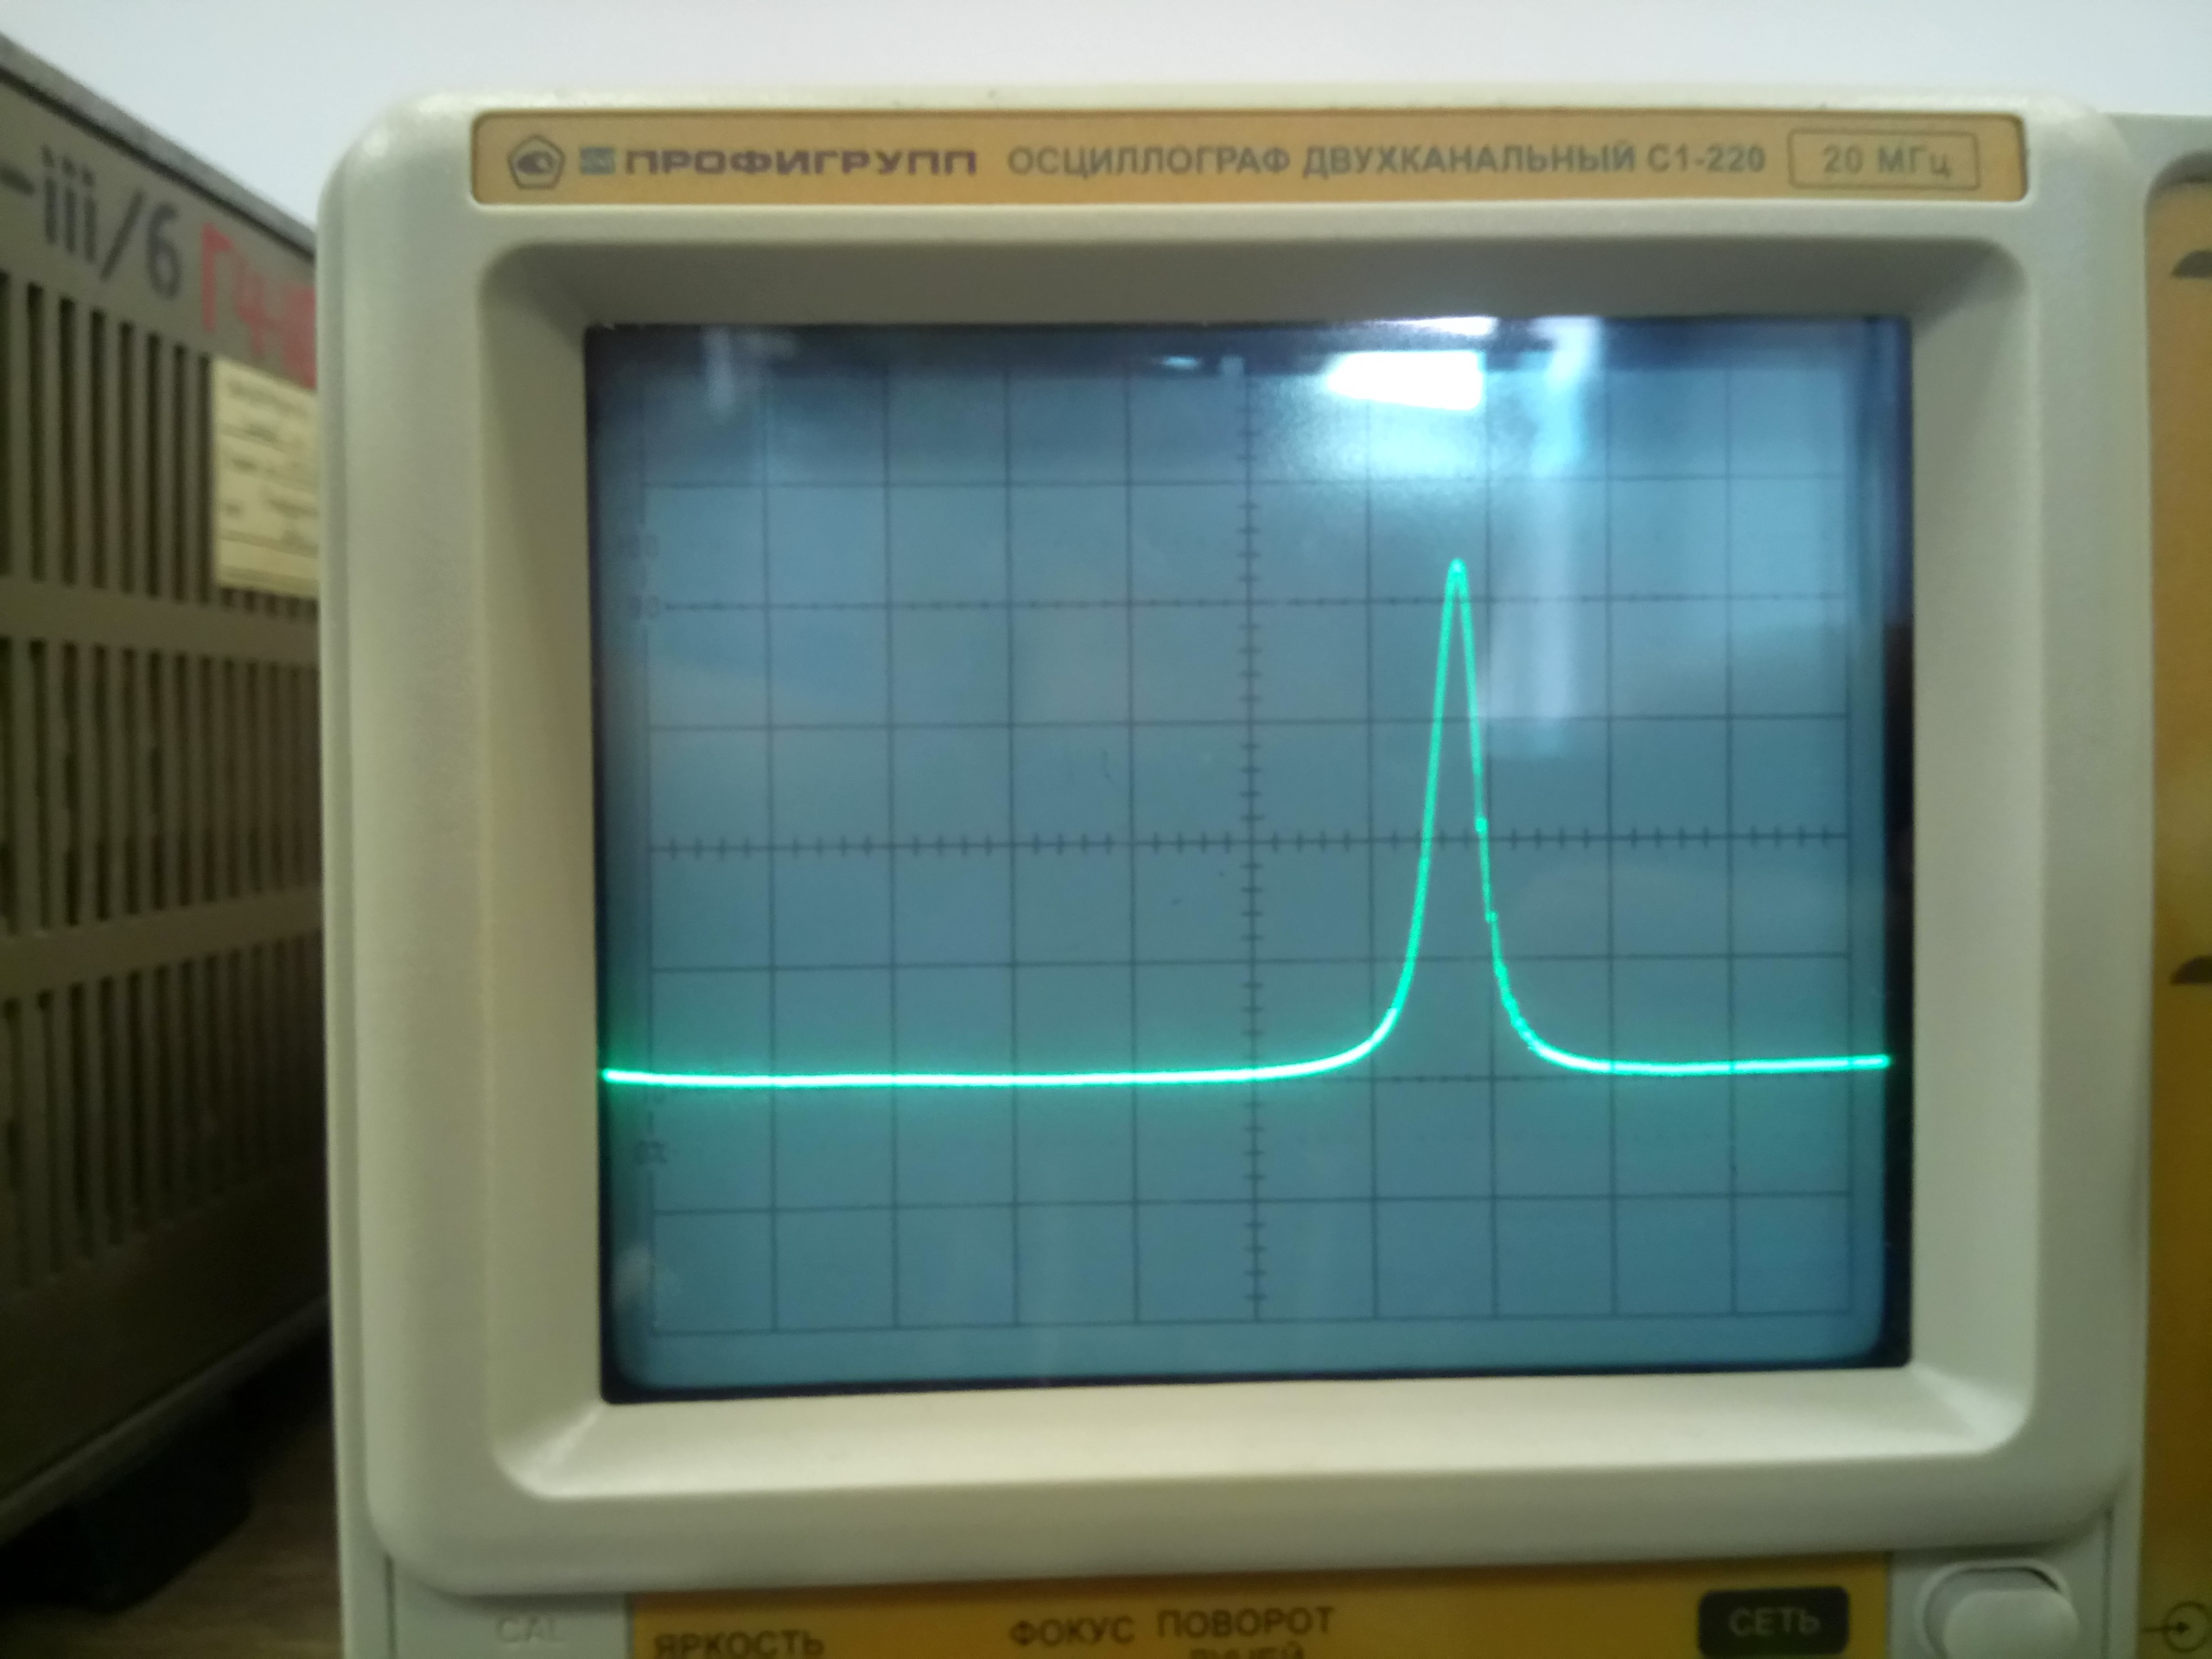
\includegraphics[width=0.3\linewidth]{fig/fig3}
    \caption{Характерная осциллограмма при ЭПР(а), кривая $\chi'$ (б), кривая $\chi''$ (в)}
    \label{fig:2}
\end{figure}

Для получения кривых $\chi'$ и $\chi''$, в соответствии с формулой \eqref{eq:14} (при $\alpha = 0$) перемещался плунжер балансного плеча. Полученные осциллограммы
приведены на рис. \ref{fig:2}(б,в).

\paragraph{Измерение ширины линий поглощения сигнала ЭПР в единицах поля.}%
Для получения ширины линии, шкала осциллографа была проградуирована по единицам поля (21.88
Гс/кл). Ширина линии поглощения $\chi''$ на половине высоты 
$$\Delta H = 10.9 ~\delta H$$

\paragraph{Расчет ширины линии в единицах частоты.}

\paragraph{Определение числа парамагнитных частиц в образце.}%
Для вычисления числа парамагнитных частиц, воспользуемся пунктом \ref{sub:2} теории и формулой \eqref{eq:21}.
\begin{equation}
    \label{eq:21a}
    N_0 = \frac{3KT}{8 \pi Q \mu^2 \omega_0 T^*_2} \cdot \frac{L_C}{L_M} \cdot \frac{P_M}{P_n} \cdot \frac{V_{\text{рез}}}{V_{\text{обр}}},
\end{equation}
где $T_2^*$ -- время поперечной релаксации,  $K$ -- постоянная Больцмана,  $\mu$ -- магнитная проницаемость дифенила,

Свыше нам даны следующие величины:
\begin{equation}
    \label{eq:}
    Q = 5000, \quad \frac{V_{\text{рез}}}{V_{\text{обр}}} \simeq 200, \quad \frac{P_M}{P_n} = 1
\end{equation}

Из эксперимента остается определить собственную частоту резонатора $\omega_{0}$ (нашли в \ref{par:1}.3), время поперечной релаксации $T^*_2$ и отношение  $L_C / L_M$ (нашли двумя параграфами выше). 

\end{document}
